\chapter{Results: Alpine Species Suitability Graphs} \label{AppendixI}

\begin{figure}[htb!]
\center
	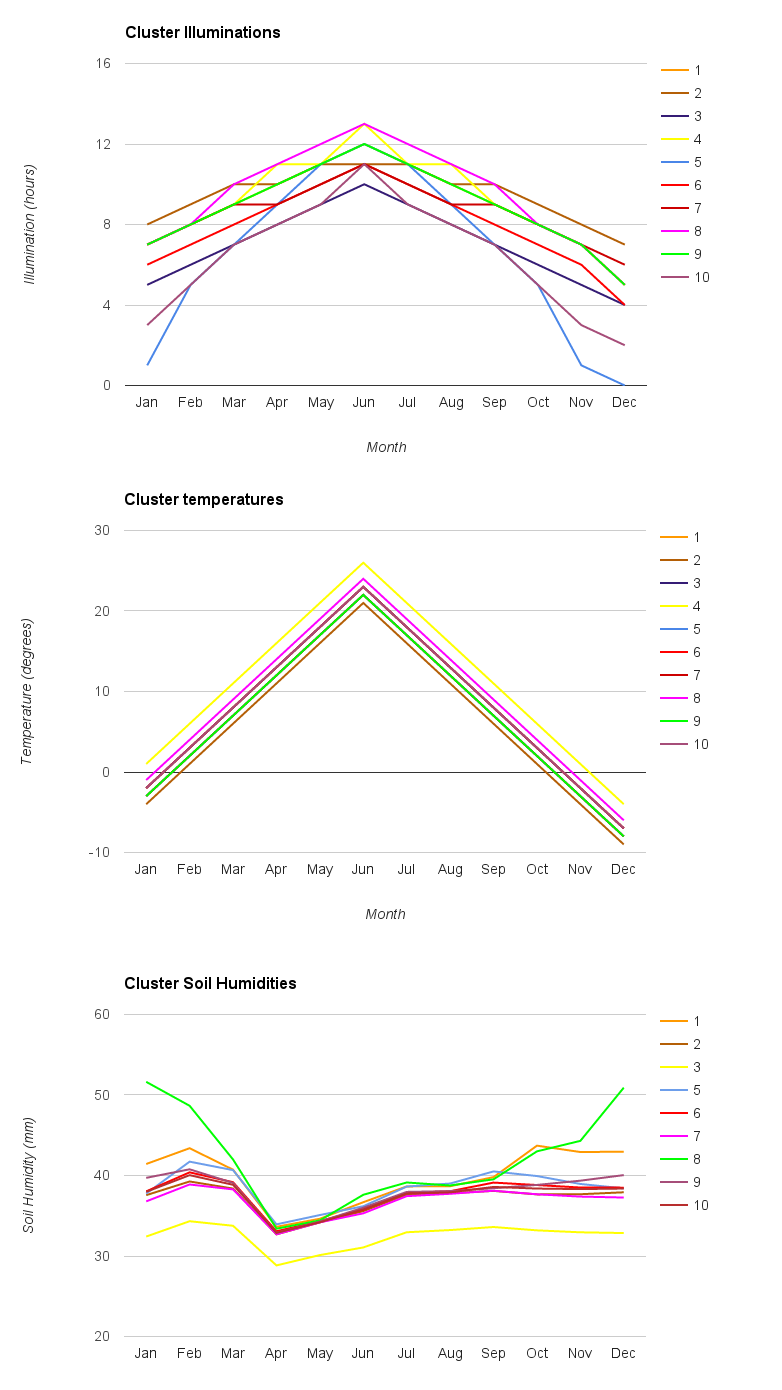
\includegraphics[height=\textheight-60pt,keepaspectratio]{results_alpine_clusters_hum_illum_temp.png}
	\caption{ \textit{Alpine: Mean monthly sun exposure (top), temperatures (middle) and soil moistures (bottom) for each terrain cluster. Note that soil humidity data is removed for cluster 4 because the values are too high.}}
	\label{fig:results_alpine_cluster_hum_temp_illum}
\end{figure}

\begin{figure}[htb!]
\center
	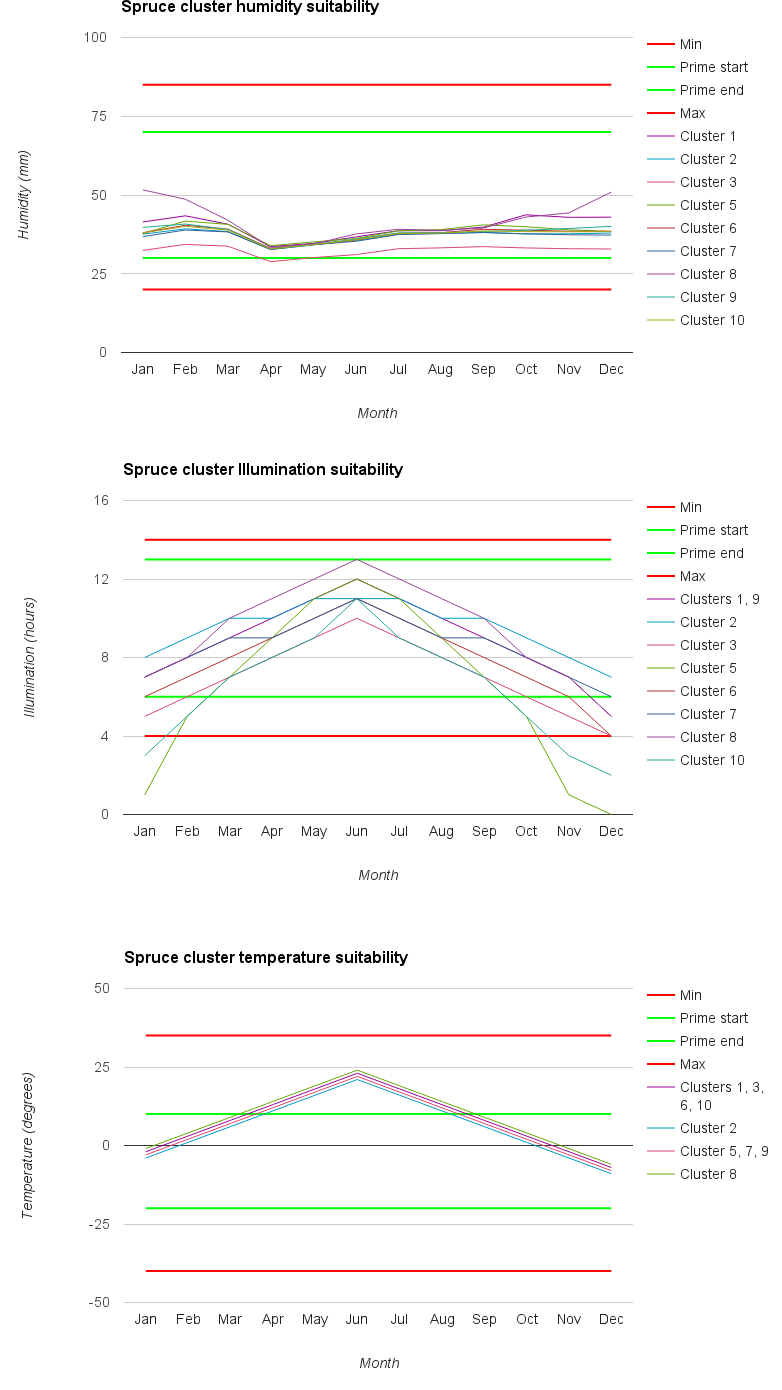
\includegraphics[height=\textheight-60pt,keepaspectratio]{spruce_suitability.png}
	\caption{ \textit{Alpine: Spruce suitability to clusters 1, 2, 3, 5, 6, 7, 8, 9 and 10 in terms of temperature (top-left), illumination (top-right) and soil humidity (bottom). The thick green lines and red lines delimit the species prime range and absolute limits respectively.}}
	\label{fig:results_alpine_spruce_suitability}
\end{figure}

\begin{figure}[htb!]
\center
	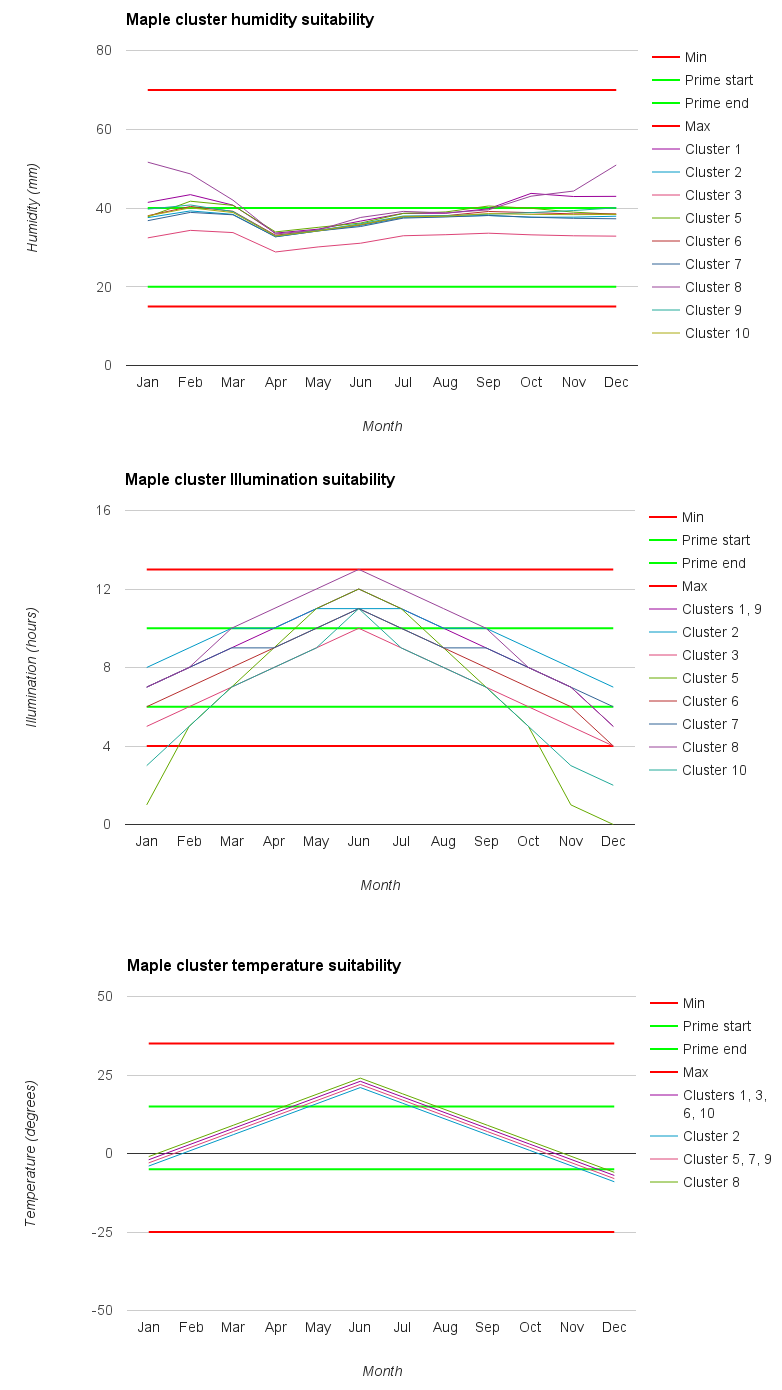
\includegraphics[height=\textheight-60pt,keepaspectratio]{maple_suitability.png}
	\caption{ \textit{Alpine: Maple suitability to clusters 1, 2, 3, 5, 6, 7, 8, 9 and 10 in terms of temperature (top-left), illumination (top-right) and soil humidity (bottom). The thick green lines and red lines delimit the species prime range and absolute limits respectively.}}
	\label{fig:results_alpine_maple_suitability}
\end{figure}

\begin{figure}[htb!]
\center
	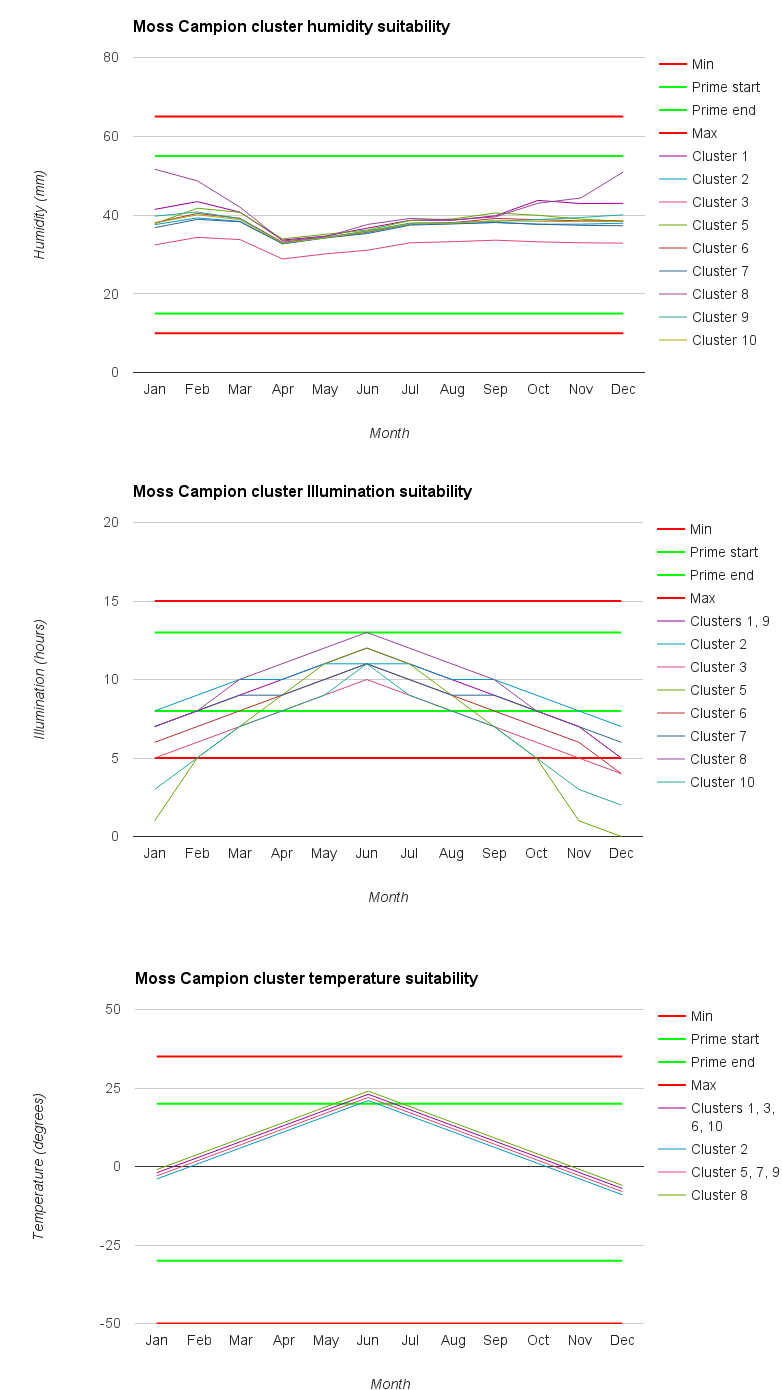
\includegraphics[height=\textheight-60pt,keepaspectratio]{moss_campion_suitability.png}
	\caption{ \textit{Alpine: Moss Campion suitability to clusters 1, 2, 3, 5, 6, 7, 8, 9 and 10 in terms of temperature (top-left), illumination (top-right) and soil humidity (bottom). The thick green lines and red lines delimit the species prime range and absolute limits respectively.}}
	\label{fig:results_alpine_moss_campion_suitability}
\end{figure}

\begin{figure}[htb!]
\center
	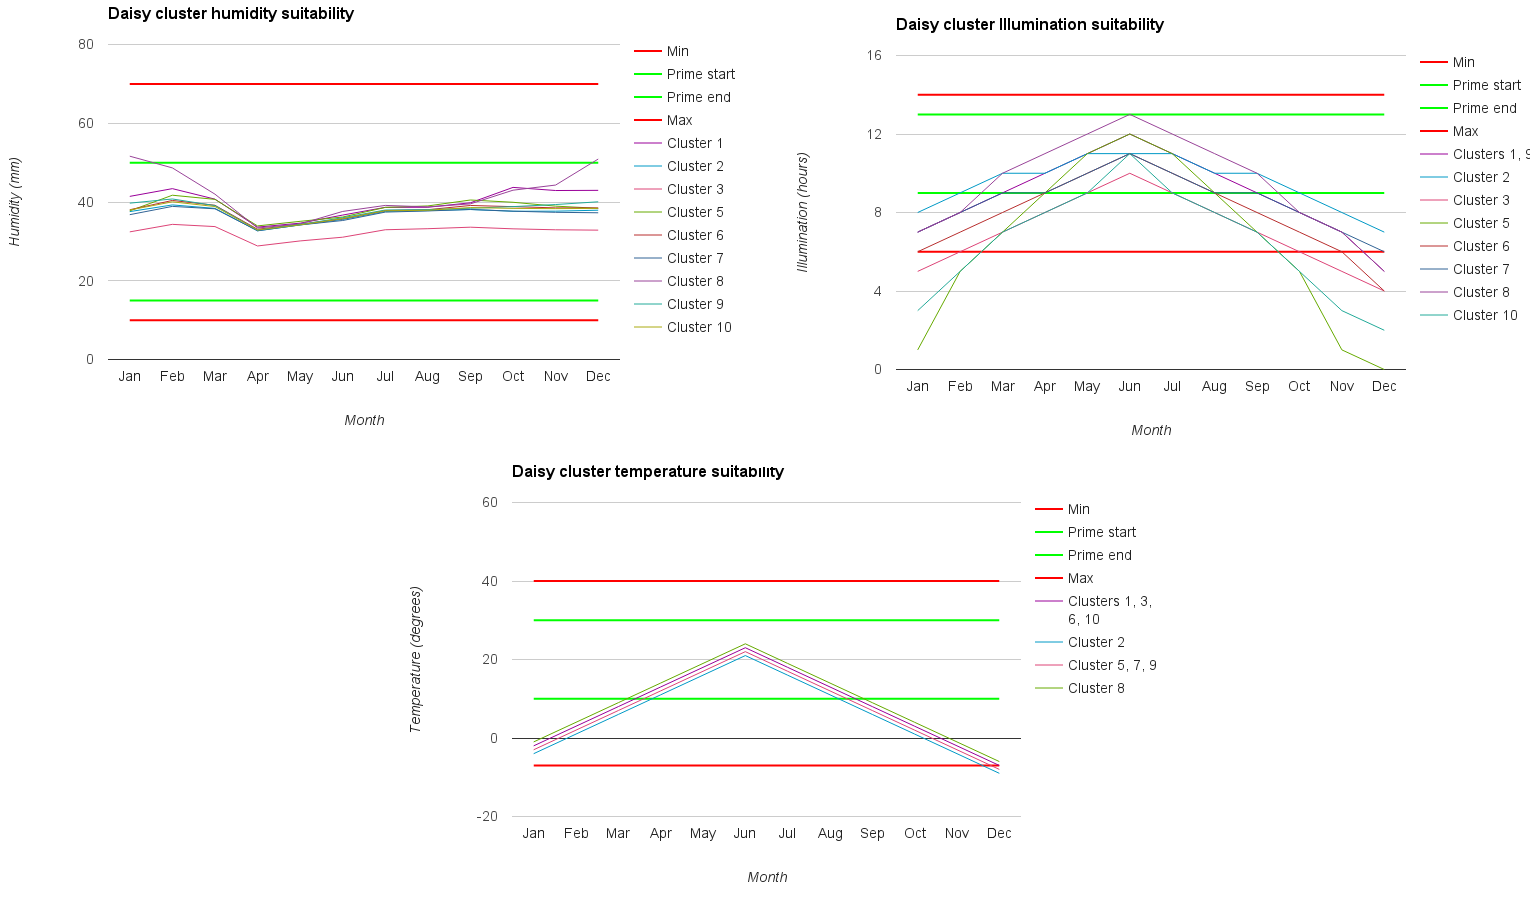
\includegraphics[height=\textheight-60pt,keepaspectratio]{daisy_suitability.png}
	\caption{ \textit{Alpine: Daisy suitability to clusters 1, 2, 3, 5, 6, 7, 8, 9 and 10 in terms of temperature (top-left), illumination (top-right) and soil humidity (bottom). The thick green lines and red lines delimit the species prime range and absolute limits respectively.}}
	\label{fig:results_alpine_daisy_suitability}
\end{figure}

\begin{figure}[htb!]
\center
	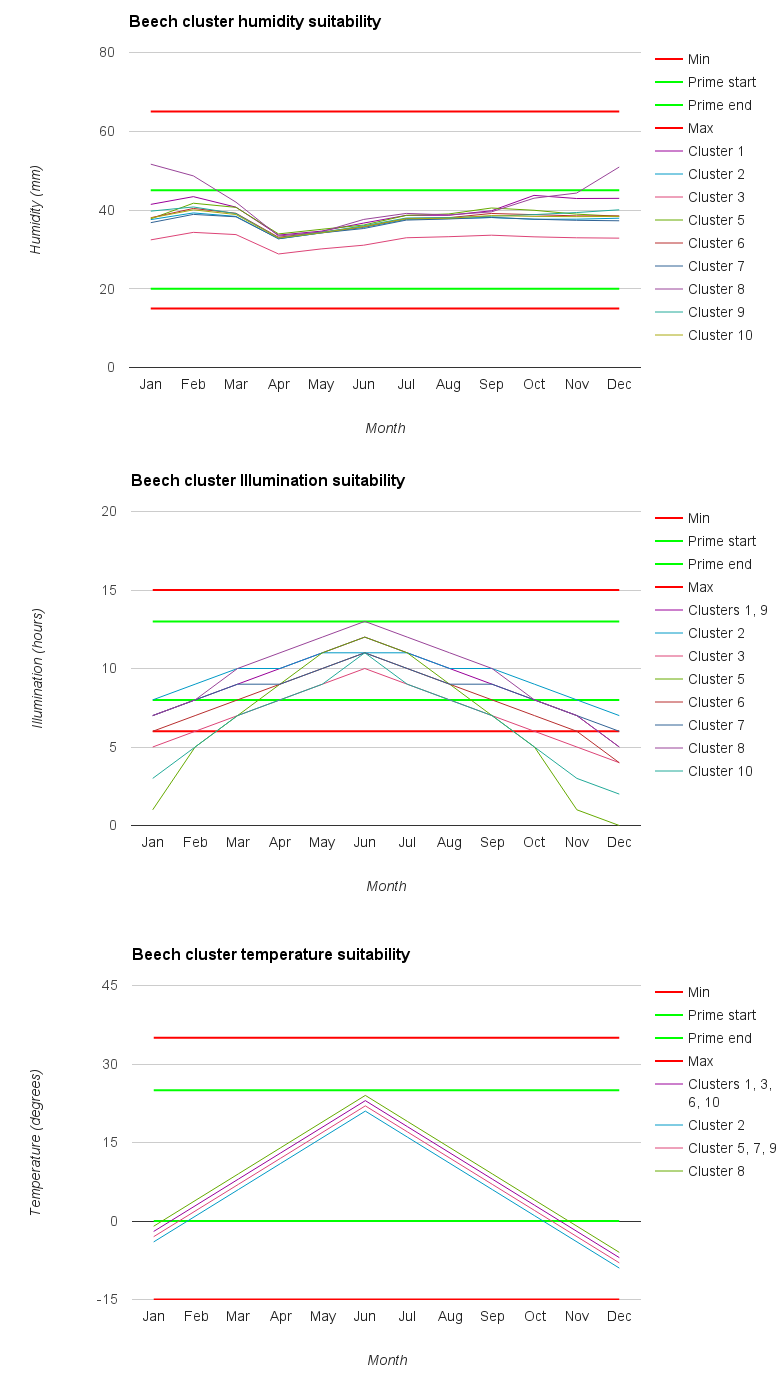
\includegraphics[height=\textheight-60pt,keepaspectratio]{beech_suitability.png}
	\caption{ \textit{Alpine: Beech suitability to clusters 1, 2, 3, 5, 6, 7, 8, 9 and 10 in terms of temperature (top-left), illumination (top-right) and soil humidity (bottom). The thick green lines and red lines delimit the species prime range and absolute limits respectively.}}
	\label{fig:results_alpine_beech_suitability}
\end{figure}